\section{Method}
\label{sec:problem}

We choose an optimal summarization of the knowledge evolutionary trend base on \emph{content coverage} and \emph{ burstiness} of words, the method yields intuitive coarse-level summarization of the temporal dynamics of a given research topic.

The four-step approach are summarize as below:

\textbf{Step.1 Expert finding}
We use a community-based summarization as we first find a core community (a group of experts) related to the topic, and then aggregate each member's research work as the documents to summarize. To avoid some authoritative experts dominate the research area and introduce potential bias, we normalize each member's contribution averagely.

\textbf{Step.2 Knowledge concept extraction}
With the retrieved document collection, we extract terms mentioned in each document and construct a network $G$, where a term $w_i$ appears in a time slide $t$ is associated with a node $n_i^t$.
\begin{center}
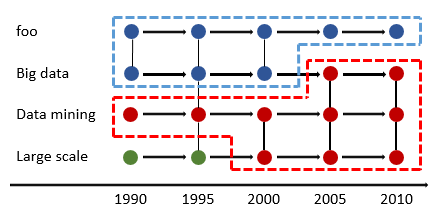
\includegraphics[width=0.80\linewidth]{figures/mutual.png}
\end{center}
There are two types of edges in the graph:

\begin{itemize}	
\item The concepts in the same time slide are connected with mutual info edge. For an arbitrary edge $(n_i^t, n_j^t)$, the weight from $n_i^t$ to $n_j^t$ is $W(n_i^t,n_j^t) = \frac{I(n_i^t,n_j^t)}{I(n_i^t,n_i^t)}$, where $I(n_i^t,n_j^t)$ indicates the mutual information between $w_i$ and $w_j$ within the time slide $t$.
\item Nodes corresponding to the term $w_i$ within two adjacent time slides $t$ and $t+1$ are connected by an evolving edge $(n_i^t,n_i^{t+1})$, indicates the knowledge concept is evolved from itself in the last time slide. The weight of the evolving edge is a parameter controlling the temporal smoothness of the summarization.
\end{itemize}

\textbf{Step.3 Knowledge concept selection}
The following task is to choose a set of terms best summarize the whole research area. We use two measures: \emph{Coverage} and \emph{Burstiness} to choose the terms of interest.

\begin{itemize}
\item We model burstiness by assuming the arrival of words as a unknown binomial distribution, and use $\chi^2$ tests to check for significant association between word and time periods. We calculate the contingency table as below and $\chi^2 = \frac{(ad-bc)^2n}{(a+b)(c+d)(a+c)(b+d)}$.
\begin{center}
\begin{tabularx}{0.5\linewidth}{ |X|X|X| }
  \hline
  - & $W$ & $\bar{W}$ \\
  \hline
  $t$  & a  & b  \\
  \hline
  $<t$  & c  & d  \\
  \hline
\end{tabularx}
\end{center}

\item We use a influence maximization based model to model information coverage of terms. More specifically, we use a linear threshold model, where influence probability from $n_i^t$ to $n_j^t$ is defined as $$P_{i,j}^{t} = \alpha P_{i,j}^{t-1} + (1-\alpha)W(n_i^t, n_j^t)}$$, and the activate threshold of $n_i^t$ is $$\Theta_i^t = \beta \Theta_i^{t-1} + (1-\beta) e^{\sum wX}$$, where $X$ is a feature vector and $w$ is the weight. The problem is to choose a set of $k$ term that maximize the content coverage. 

\end{itemize}

\textbf{Step.4 Trend partitioning}
After choosing a set of summarization words, we further grouping the rest of the words into clusters, and finally we can use the clusters over time to indict evolving trend and generates the highly intuitive visualization.
